
%(BEGIN_QUESTION)
% Copyright 2014 Tony R. Kuphaldt, released under the Creative Commons Attribution License (v 1.0)
% This means you may do almost anything with this work of mine, so long as you give me proper credit

A current transformer senses line current to a 3-phase load and drives a signal to a meter which contains both inductance and resistance:

$$\includegraphics[width=15.5cm]{i03124x01.eps}$$

Calculate the voltage dropped across the {\it inductive} portion of the meter's burden.  Your answer needs to specify both the magnitude of this voltage as well as its phase angle:

\vskip 10pt

$V_L$ = \underbar{\hskip 80pt} 

\underbar{file i03124}
%(END_QUESTION)





%(BEGIN_ANSWER)

$V_L$ = 1.563 V $\angle$ $110^o$ 
 
%(END_ANSWER)





%(BEGIN_NOTES)


%(END_NOTES)


